\thispagestyle{only-cfoot}
\section{Introduction to problem domain}\label{s:ProblemDomain} % Problem background

This chapter contains a short introduction to problem-related terms and concepts referred to further in this work.
It begins with a high-level overview of the Kubernetes platform in section \ref{s:ProblemDomain:Kubernetes} and cloud computing with its services in section \ref{s:ProblemDomain:Cloud}.
The section \ref{s:ProblemDomain:Scheduling} provides an overview of known scheduling approaches and algorithms and explains the task clustering phenomenon.
Sections \ref{s:ProblemDomain:Workflow} and \ref{s:ProblemDomain:Hyperflow} describe the ideas of scientific workflows and workflow management systems and cover the introduction to Hyperflow system.


\subsection{Kubernetes}
\label{s:ProblemDomain:Kubernetes}

One of the most advanced and popular container management tools available today is \emph{Kubernetes}, a platform for container orchestration it is often used in vast range of projects with virtualized work environments.
It is a next-generation successor \cite{b:Borg-K8s-predecessor} to a Borg cluster manager.
Within its responsibilities lies e.g. resource allocation, container monitoring and handling failovers.
Being an open-source solution it is also extensible \cite{b:Kubernetes-what-is}, which enables the user to integrate their own custom extensions over a predefined interface to adjust core funcitonalities to their needs. A top level architecture of Kubernetes cluster is presented in \cref{fig:kubernetes:architecture} and consists of a control plane that serves a role akin to the cluster's master node, and worker nodes.

%%%%
\begin{figure}[H]
\centering
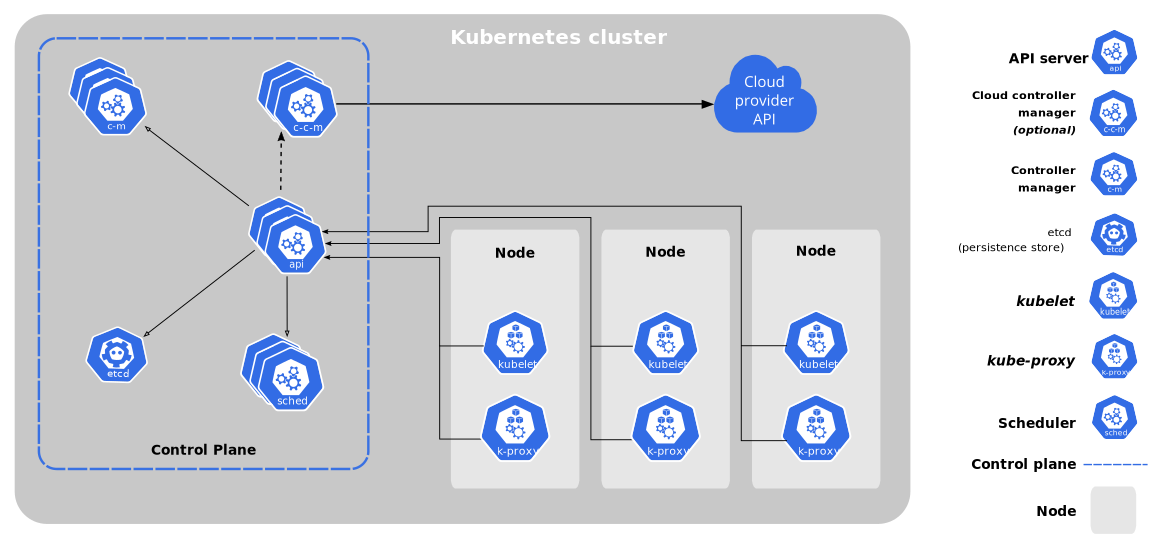
\includegraphics[width=1\linewidth]{figures/2-1-k8s-arch.png}
\caption[Kubernetes cluster architecture diagram]{A diagram\footnotemark of Kubernetes cluster components and processes distributed among them.}

% \medskip
% \begin{minipage}{0.65\textwidth}
% {\footnotesize Depicts Kubernetescluster components and processes distributed among them.\par}
% \end{minipage}

\label{fig:kubernetes:architecture}
\end{figure}
\footnotetext{Source: \url{https://kubernetes.io/docs/concepts/overview/components}, Access: 2021-05-26}
%%%%

With an exposed \emph{Application Programmable Interface (API)} workloads can be dynamically scheduled by any authorized third-party application.
They are represented in a form of a configuration file called \emph{deployment}, which contains details for requested Kubernetes resources such as pods or services.

%%%%%%%



\subsubsection{Pod}\label{s:ProblemDomain:Kubernetes:pod}

A base workload type in Kubernetes is called \emph{pod} and is meant to represent a standalone working process. 
It is used as an abstraction for a set of tightly-coupled containers required to be scheduled on the same worker node.
Although the requests for computing resources for each of the containers within a single pod may differ, they still share the storage with themselves.
In most cases though, a single pod comprises of only one container.

%%%%%%%



\subsubsection{Job}\label{s:ProblemDomain:Kubernetes:job}

Another workload type available is Kubernetes \emph{job}.
This one abstracts the group of pods that should be run together to execute one specific task.
Jobs are often used in situations where there is a need to run a task with a limited execution time and track its completion status and result data.
Also they ensure completion of the task, monitoring statuses of the assigned pods and rescheduling those that have erred until the required number of them have successfully completed.

%%%%%%%



\subsubsection{Kube-scheduler}\label{s:ProblemDomain:Kubernetes:scheduler}

In Kubernetes the responsibility of pod allocation and node assignment belongs to \emph{kube-scheduler}.
The procedure used to determine which node to choose for a specific pod comprises of two actions -- \emph{filtering} and \emph{scoring} \cite{b:Kubernetes-scheduler}.
Filtering process selects candidate nodes that meet pods resource requirements.
When there are no such nodes available at a given moment the scheduled pod must wait for allocation until there is at least one candidate node.
The candidate nodes are then evaluated in the scoring process which determines the best-fitting node for the pod.

It is possible to adjust the scheduler decisions to match the users expectations. 
To limit the possible candidate nodes a pod may have configured additional constraints along its resource requirements.
One of them are node selectors which limit the pool of nodes to those that have defined a specific label on them.
The default Kubernetes scheduler also offers a few scheduling policies to choose from that affect the scoring process.
Additionally, users may also implement their own scheduler components and use them instead of the kube-scheduler \cite{b:Kubernetes-scheduler}.
The only limitation is the new scheduler needs to maintain the filtering and scoring behaviour as a part of the interface.

%%%%%%%


\subsection{Cloud computing}
\label{s:ProblemDomain:Cloud}

The term \emph{cloud computing} is used to describe a group of services with elastic pool of resources available to the end users \emph{on-demand} and settleable based on their usage quota \emph{(pay-as-you-go)} \cite{b:Cloud-Principles-Paradigms}.
In order to distinguish different cloud services they are often classified by their abstraction level as specific service models with the three main being:

\begin{itemize}
  \item{
\emph{Software as a Service (SaaS)} -- the primary resources are provider's applications that run and are managed, transparently to the user
};
  \item{
\emph{Platform as a Service (PaaS)} -- enables deployment of users applications on computing units which abstracts actual physical resources from user, preventing any interaction with underlying infrastructure
};
  \item{
\emph{Infrastructure as a Service (IaaS)} -- a model where users have to configure and manage the infrastructure by themselves, where the base resources are e.g. virtual machines, data storage and network components.
}
\end{itemize}
The abstraction level of a service is related to the number of intermediary layers between the final resource and physical infrastructure.



\subsubsection{Container as a Service}
\label{s:ProblemDomain:CaaS}

Another model of cloud services available in today's clouds is \emph{Container as a Service (CaaS)}.
Relating it to other service models it is classified as one in between of the IaaS and PaaS \cite{b:IBM-CaaS}.
With containers being treated as a primary resource it enables interaction with infrastructure at a higher abstraction level than in IaaS, nonetheless the responsibility for the management process still lies in hands of the end user.
This model offers a more scalable and portable solution to infrastructure management for containerized environments.



\subsubsection{Elastic Kubernetes Service}
\label{s:ProblemDomain:EKS}

An example of an CaaS service is \emph{Elastic Kubernetes Service (EKS)} \cite{b:IBM-CaaS} provided by \emph{Amazon Web Services (AWS)}.
It allows configuration of fully-managed Kubernetes cluster \cite{b:AWS-EKS} in AWS cloud environment.
This means that EKS by itself spans a new cluster, covers the Kubernetes installation process and is responsible for maintaining the Kubernetes control plane outside the cluster's nodes.
The end user is only responsible for initial cluster configuration and requesting workloads on the cluster with Kubernetes API.

\subsection{Workflow}
\label{s:ProblemDomain:Workflow}

Workflow is an application comprising of a set of tasks, where some of them are dependent one on another and all need to be processed in order to complete the workflow's objective and yield the final results.
Each job in such a pipeline may require its own input data to begin execution and returns an output when it ends successfully.
As tasks cannot start without their input, they need to wait for results from other tasks, which creates a dependency relationship.
This allows such applications to be represented in the form of a \emph{Directed Acyclic Graph (DAG)} as shown in \cref{fig:workflow:dag-example}.

Furthermore, not all the jobs in a workflow must perform the same set of operations at runtime.
The pipeline has a layered structure where each layer represents a group of tasks independent of each other.
This allows for a straightforward data-parallel task execution within a single layer. 


%%%%
\begin{figure}[H]
\centering
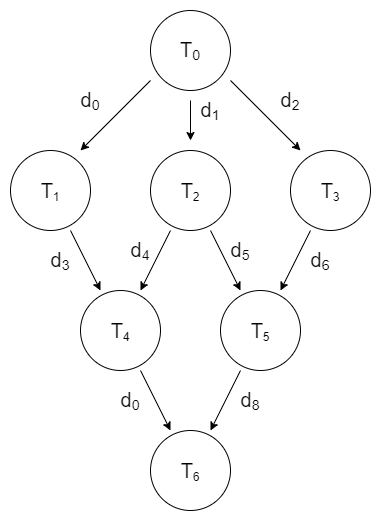
\includegraphics[width=0.3\linewidth]{figures/2-3-dag-example-with-d.png}
\caption[Exemplary workflow application structure]{Exemplary workflow application structure. Tasks are presented as a \emph{T\textsubscript{i}} nodes and dependencies as a \emph{d\textsubscript{j}} edges.}
\label{fig:workflow:dag-example}

% \smallskip
% \begin{minipage}{0.6\textwidth}
% {\footnotesize
% Tasks are presented as a \emph{T\textsubscript{i}} nodes and dependencies as a \emph{d\textsubscript{j}} edges. 
% \par}
% \end{minipage}

\end{figure}
%%%%


There are applications with more than one starting or finishing job, however their representations can have single abstract nodes prepended or appended, in order to match the input for scheduling algorithms.



\subsubsection{Montage}

One of the scientific workflows integrated with Hyperflow system is \emph{Montage}.
It is a toolkit that provides transformations for astronomical images to turn them into custom, science-grade mosaics \cite{b:Montage-url}.
Each transformation is provided as a separate software module \cite{b:Montage} so together they can be piped into a single workflow.



\subsubsection{SoyKB}

The \emph{Soybean Konwledge Base (SoyKB)} is a platform for storing soybean genomics datasets and providing them via an interface for research.
To analyze this data the \emph{PGen workflow} was created allowing analysis on both Linux environment and through SoyKB online submissions \cite{b:SoyKB-workflow-url, b:SoyKB-PGen}.
% The latter environment integration allows execution of the workflow with task containerization.
Being consistent with Hyperflow naming, in this work all mentions of \emph{SoyKB workflow} are in fact referring to the PGen application.




\subsection{Scheduling}
\label{s:ProblemDomain:Scheduling}

The \emph{scheduling problem} is a term referring to a process of arranging tasks and assigning them to selected processing units with goal of workload optimization, e.g. minimize completion time.
To provide a sub-optimal solutions to this NP-complete problem many heuristics have been researched and developed with two main approaches considered -- \emph{static} and \emph{dynamic} scheduling.
The final solutions can be \emph{workflow-aware} which means they take the dag-oriented structure of the workload into consideration during task arrangement.


\subsubsection{Static scheduling}
\label{s:ProblemDomain:StaticSched}

In static scheduling, it is assumed that all requirements are already defined, including task resource demands and information about execution environment with underlying infrastructure.
This approach allows to optimize the workload distribution across all of the computing units.
At the same time it lacks the adaptability to unforeseen changes in resource availability. 


There are multiple categories of static scheduling algorithms, one of them being a \emph{list-based} ones.
The \emph{list-based} algorithms consist of two phases:


\begin{itemize}
  \item{
\emph{prioritization} -- during this phase each task has its the \emph{rank} value calculated and has its priority based off of it. The tasks are then ordered descendingly by their priorities
};
  \item{
\emph{selection} -- in this stage the final sequences of tasks are formed, one for each available computing unit. A sequence binds the tasks to a selected processor and defines their execution execution order that must be followed.
}
\end{itemize}


An example of list-based workflow scheduling algorithm is \emph{Heterogeneous Earliest Finish Time (HEFT)}, where the rank of a task is based on the its computation and communication costs \cite{b:HEFT}.
Another algorithm worth mentioning is a \emph{Predict Earliest Finish Time (PEFT)}.
Despite both algorithms using same parameters in rank calculation process, they have different formulas defined.
The difference comes from PEFT's \emph{Optimistic Cost Table (OCT)} which is used to evaluate the future impact of assigning a given task to specific node \cite{b:PEFT}. \todo{ Może wspomnieć o wynikach porownania PEFT do HEFT z \cite{b:PEFT} ?}



\subsubsection{Dynamic scheduling}
\label{s:ProblemDomain:DynamicSched}

The dynamic approach to scheduling problem concentrates more on an issue of changeability of computing environment, availability of its resources and changes to processors load.
All scheduler's decisions are being made at runtime based on information know only at the exact moment in time.
This makes them more adaptable, but at the same time there is a disadvantage of worse workload optimization than with static scheduling \cite{b:Dynamic-Scheduling-Case-Study}.
Additionally, the dynamic nature makes it a go-to approach for cluster schedulers \cite{b:Tetris, b:Graphene}.



\subsubsection{Task clustering}
\label{s:ProblemDomain:TaskClustering}

Executing a lot of short tasks in a single limited computing environment leads to increase in slowdown and decrease in overall resource utilization.
To address this problem the \emph{task clustering} solutions are used.
The idea behind them is to group the waiting tasks into the multi-element clusters and treat them as a single entity \cite{b:Task-Clustering-Pegasus} during the scheduling process.

There are various approaches to clustering tasks in a workflow.
The ones related to granularity problem are:


\begin{itemize}
  \item{
\emph{horizontal} -- also called a \emph{level-based}, is a clustering solution that forms groups based on the task level of in workflow's DAG representation. In horizontal approach clusters can be composed of entities with the same level
};
\item{
\emph{vertical} -- tasks are grouped only vertically with the child tasks dependent on them or the parent tasks they are dependant on. The problem with vertical clustering is the task resource requirements in the same cluster may differ
};
  \item{
\emph{label-based} -- in this approach all tasks are being labeled by the end user and grouped with other ones that have the same label. Then all the tasks within a single cluster have to be ordered for an execution \cite{b:Task-Clustering-Hybrid-Algorithm, b:Task-Clustering-Pegasus}.
}
\end{itemize}


% Moze przeniesc do osobnej subsection, niekoniecznie zwiazany z schedulingiem ?


\subsection{Hyperflow}
\label{s:ProblemDomain:Hyperflow}

\emph{Workflow Management System (WMS)} is a software responsible for coordinating and supervising workflow execution.
It provides storage layers for data exchange, manages states of the workflow's tasks and handles permissions for waiting jobs to allow them to run only when their dependencies are fulfilled.
One of such systems is \emph{Hyperflow} -- an innovative yet lightweight and simple model for workflow execution \cite{b:Hyperflow}.
Its two main constituents are an engine, which makes all the decisions regarding workload allocation, and an executor that handles assigned workloads within separate processes, monitors their status and reports completion to the engine.


Executors are the supervisors spawned by an engine using a concept Hyperflow functions.
With each one implementing a different workload deployment solution for a specific kind of infrastructure Hyperflow can be used in various computing environments including Kubernetes clusters \cite{b:Hyperflow-k8s-deployment}.
The \cref{fig:hyperflow:architecture} presents an overview of a system architecture in a Kubernetes environment.
Each workflow's task is considered as a separate workload and is represented by a single Kubernetes job.
Its deployement is being requested by the Hyperflow engine through a function that calls the cluster's API.


%%%%
\begin{figure}[H]
\centering
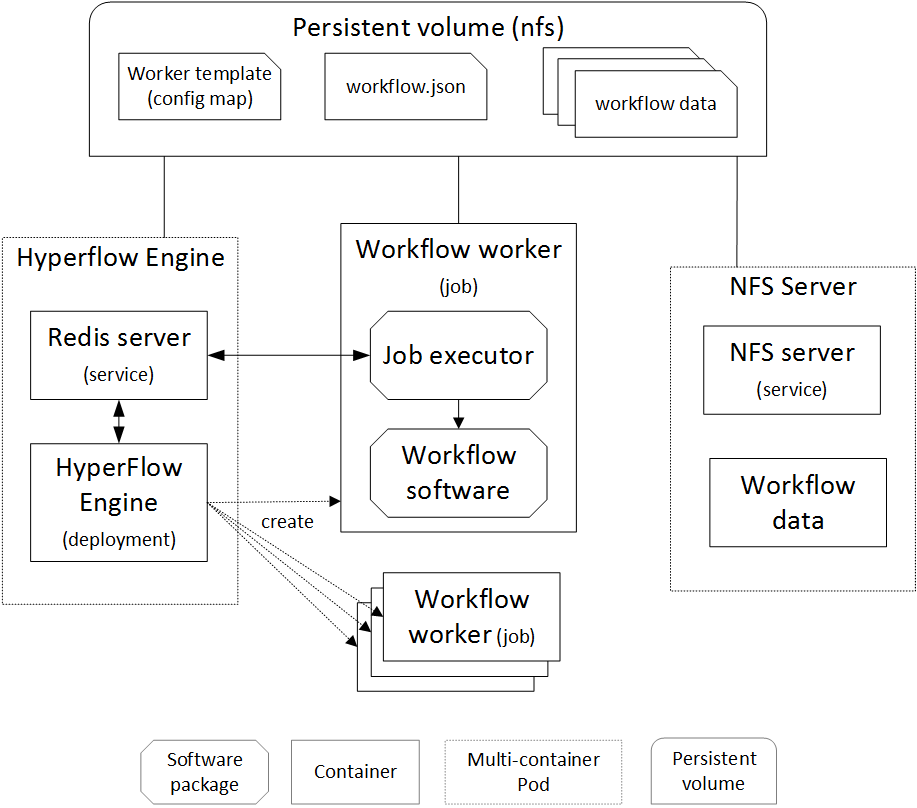
\includegraphics[width=0.6\linewidth]{figures/2-4-hyperflow-k8s-arch.png}
\caption{Hyperflow architecture in Kubernetes cluster}

\smallskip
\begin{minipage}{0.7\textwidth}
{\footnotesize\centering
SOURCE: \cite{b:Hyperflow-k8s-deployment}
\par}
\smallskip
{\footnotesize
One of the cluster's nodes is reserved to be a Hyperflow master node.
Engine's components are deployed on the master node, while tasks are deployed with their executors on the worker nodes.
Workflow data is being exchanged through network file system.
\par}
\end{minipage}

\label{fig:hyperflow:architecture}
\end{figure}
%%%%

The engine allows the tasks performing the same operations to be grouped together and buffered, waiting to be assigned to a single executor instance.
Whenever a task becomes ready to be processed it is being either assigned to a new buffer or is being appended to already existing one, associated with this specific task's operation.
This feature is an implementation of a horizontal task clustering solution and is referred to as \emph{task agglomeration} in Hyperflow nomenclature.

Buffers have configurable maximum sizes and have defined time boundaries for them to wait until they are deployed as a Kubernetes job.
They allow grouping until they are already full or the timeout has been reached.
Such configurations are possible for each workflow's operation.


